\documentclass{standalone}
\usepackage{tikz}
\begin{document}
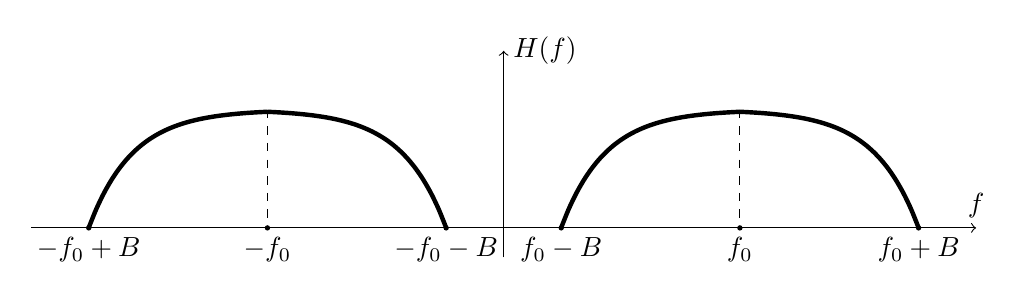
\begin{tikzpicture}[scale=1.5]
    \draw[->](-4,0)--(4,0)node[above]{$f$};
    \draw[->](0,-0.25)--(0,1.5)node[right]{$H(f)$};

    \draw[ultra thick]plot[smooth, domain=2:3.513](\x,{1-0.25*e^(2.7*(\x-3))});
    \draw[ultra thick]plot[smooth, domain=0.487:2](\x,{1-0.25*e^(-2.7*(\x-1))});
    \draw[dashed](2,1)--(2,0)node[below]{$f_0$};
    \node[below]at(3.513,0){$f_0+B$};
    \node[below]at(0.487,0){$f_0-B$};
    \filldraw[black](2,0)circle(0.5pt);
    \filldraw[black](3.513,0)circle(0.5pt);
    \filldraw[black](0.487,0)circle(0.5pt);

    \draw[ultra thick]plot[smooth, domain=-3.513:-2](\x,{1-0.25*e^(-2.7*(\x+3))});
    \draw[ultra thick]plot[smooth, domain=-2:-0.487](\x,{1-0.25*e^(2.7*(\x+1))});
    \draw[dashed](-2,1)--(-2,0)node[below]{$-f_0$};
    \node[below]at(-3.513,0){$-f_0+B$};
    \node[below]at(-0.487,0){$-f_0-B$};
    \filldraw[black](-2,0)circle(0.5pt);
    \filldraw[black](-3.513,0)circle(0.5pt);
    \filldraw[black](-0.487,0)circle(0.5pt);
\end{tikzpicture}
\end{document}